\label{chap:moses}

\todo{This whole chapter is VERY dense and VERY technical. I will have to rewrite it to something more readable..... MAYBE... DAMN THERE IS NO  TIME FOR ANYTHING}

Although our initial plan was to show translation memory only to the translator, we found out that we can also use the corpus to train a model for statistical machine translation. However, we also found that despite getting quite good results from the translation, the durations for getting the translations were too long, compared to the translation memory.

In this chapter, we will describe, how we trained the models, our results and how we managed to get the time cost down. The final model is a part of our project; the script to produce the model from the aligned data is not included, since it would require changes to EMS source code\footnote{EMS is the Experiment Management System, a system for managing Moses experiments, \url{http://www.statmt.org/moses/?n=FactoredTraining.EMS}}, which are untested at the moment and beyond the scope of this project.

Since we focus mainly on English to Czech translation, we modeled, trained and tested only for this way of translation. Training for the opposite way of translation would be possible, too, but all the necessary resources would double, while it would only benefit a small number of people.

This chapter requires some knowledge of phrase-based translation models and Moses in general. If you are not familiar with either, the short version of this chapter is that we are getting -- on subtitles -- better results with our machine translation than Google Translate, we are getting it fast, and we were able to fit it on a rather small virtual machine.


\section{Initial setup}
\subsection{Initial settings}

For training machine translation, we use our subtitle corpus, aligned by techniques described in Section~\ref{sec:aligning_subtitles}. Since we want to be more exact in this case, we used a more strict alignment, with 0.6\,s tolerance.

We do not require all the metadata about movie files for this task, so we added all the data together. We took away 15,000 sentences for MERT tuning (which proved to be too much) and 5,000 sentences for testing. The rest is training data.

Because of the way we took the testing sentences, they are all from different movies than the training data, except for at most one movie, that can have different sentences both in tuning and testing.

We run the standard EMS\footnote{EMS is the Experiment Management System, a system for managing Moses experiments, \url{http://www.statmt.org/moses/?n=FactoredTraining.EMS}} scenario on our data, which includes testing and counting BLEU score\footnote{BLEU is an automatic metric for measuring the success of a translation}. Although EMS counts both case-sensitive and case-insensitive BLEU, we chose the case-insensitive one.

We chose EMS instead of UFAL's own \texttt{eman}, simply for better documentation of the former and the inclusion of EMS in the standard Moses installation.

Initially, for the language model, we chose the IRSTLM\footnote{\url{http://hlt.fbk.eu/en/irstlm}} language model. For the translation model training, we used standard GIZA++.

We also measured the time for running the test translation.\footnote{This was achieved by adding time tracking code to the EMS source code; this code was submitted to Moses and actually ``survived'' in the main git repository for a few weeks, but was ultimately deleted, because it broke some edge cases.} Time was measured on a machine with Intel Core2 Quad CPU Q9550, with 4 cores with 2.83GHz, and 4GB of memory.

For reference on quality, we also translated the test set with Google Translate.

\begin{figure}[h]
\begin{center}
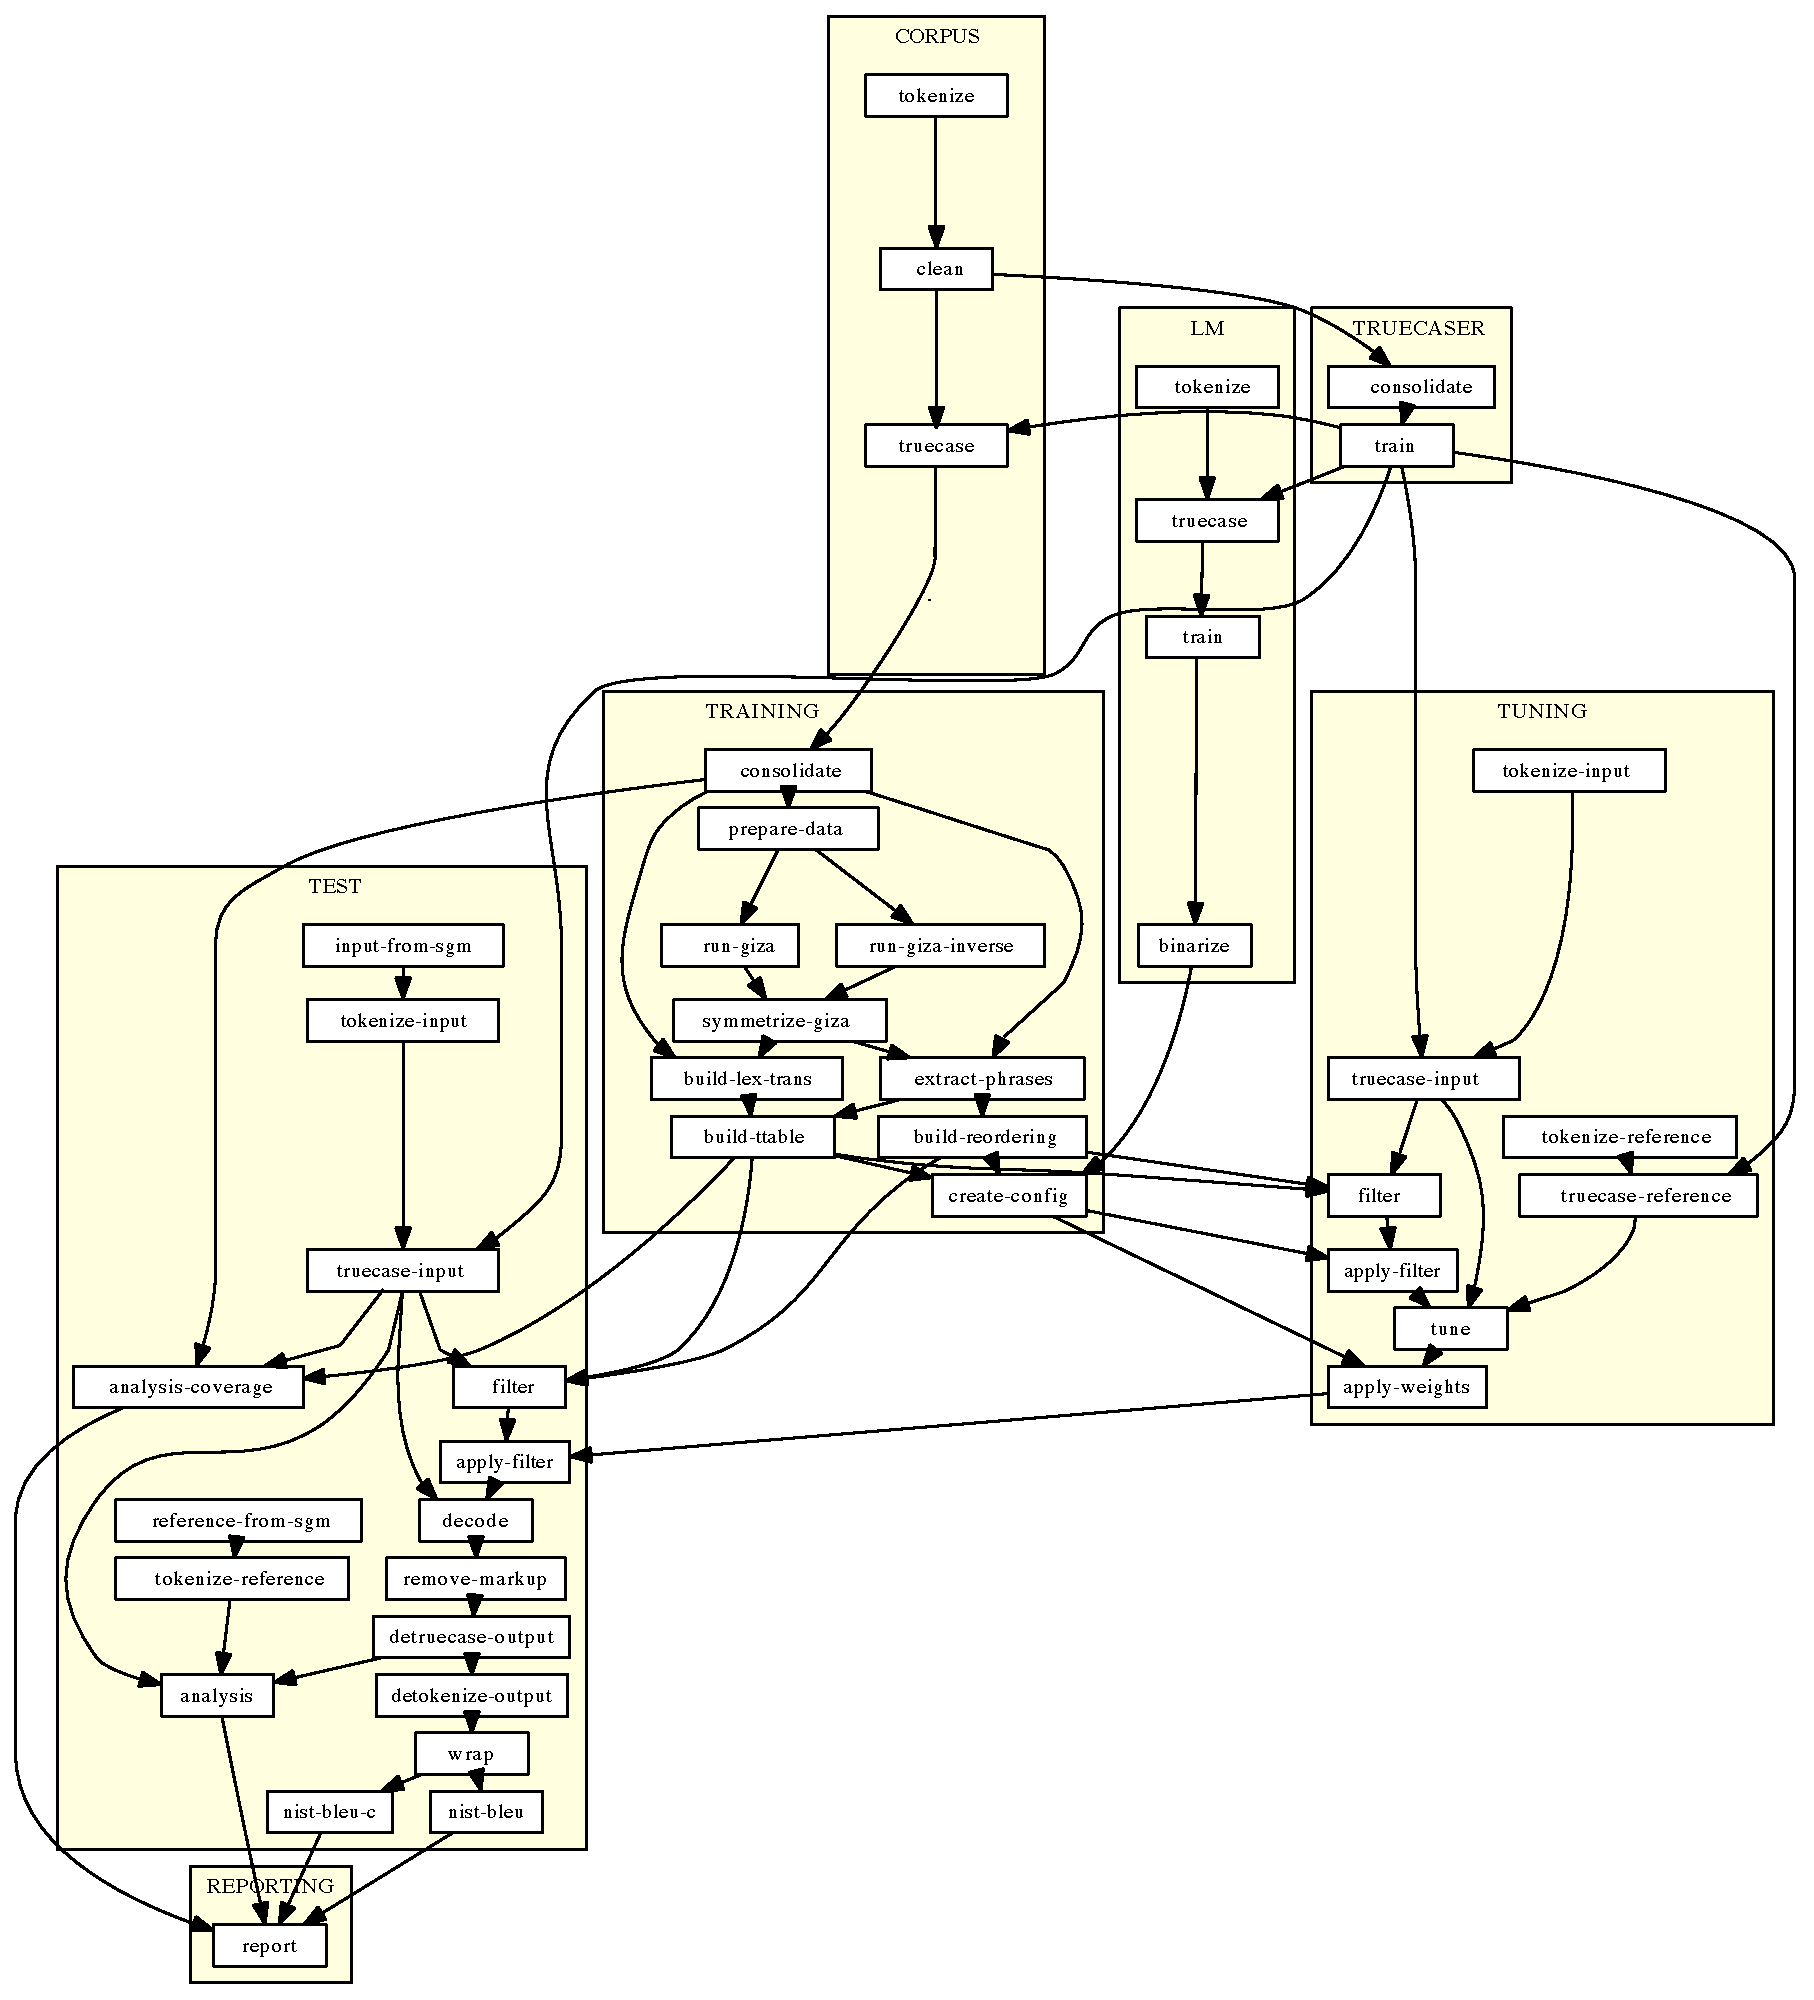
\includegraphics[width=0.8\textwidth]{figures/moses_13_graf.pdf}
\end{center}
\caption{Initial EMS set-up}\label{moses:initial}
\end{figure}

We can see the initial set-up in Figure~\ref{moses:initial}.
\subsection{Initial results}

The initial results are shown below.

\begin{table}[h]
\begin{center}
\begin{tabular}{|l|l|r|}
    \hline
    \textbf{Type} & \textbf{BLEU} & \textbf{incomplete average tps} \\ \hline
    Initial setup & 23.88 & 147\,ms \\ \hline
    Google Translate & 19.07 & N/A \\  \hline
\end{tabular}
\end{center}

\caption{Initial results (note that the time is not directly comparable with the times below thanks to the pre-filtering, as described below)}\label{moses:initialresults}
\end{table}

We were very pleasantly surprised that our initial results were better than Google Translate, without really doing anything ``smart'' on our part. This is, however, definitely caused by a smaller domain. On the \texttt{newstest2012} set, Google's results were still quite good, while ours were terribly low\todo{I don't have time to show concrete numbers now. If I have more time, will do.}; the phrases in newspapers are completely different than phrases in subtitles.

The time looked good on the first glance; however, real times observed didn't line up with the results with the model. The difference was actually caused by EMT filtering (seen on \ref{moses:initial} as ``filter''). EMT, before doing the final tests, actually filters the models in such a way that only needed parts are loaded; the actual time of the final test is, then, much lower.

Also, even when we did not optimize for time spent on initial learning, the learning phase was too long to make any experiments effective. We addressed this issue, too.

\section{Changes in the set-up}
\subsection{Tuning set size}
The biggest issue with the training was actually the MERT tuning. If we cut down the number of phrases for MERT tuning, the time for tuning decreases significantly, while the BLEU doesn't decrease that much.
\begin{table}[h]
\begin{center}
\begin{tabular}{|l|l|r|}
    \hline
    \textbf{Tuning size} & \textbf{BLEU} & \textbf{Tuning time} \\ \hline
    15,000 & 23.88 & 12 hours 57 minutes \\ \hline
    1,000 & 22.95 & 16 minutes \\  \hline
\end{tabular}
\end{center}

\caption{Tuning set size decrease}\label{moses:initialresults}
\end{table}

\subsection{Turning off the filtering}
To know the real time of the translation, we needed to turn off the filtering in EMT, which required some slight modification in the source code. 

However, after that, we found out, that unfiltered models simply will not fit into the memory of the machine. Therefore, we had to both binarize the models and prune the phrase table.

\subsection{Pruning the phrase table}
Retrieving suitable elements from the translation table takes most of the time of the entire translation task. Therefore, making it smaller would make the translation task quicker.

As a first idea, we tried to prune the phrase table by using some factoring like short stems instead of full words. However, this showed up as a dead end; too short stems produce an absolutely empty phrase table, and longer stems do not shrink the phrase table significantly.

Instead, we tried another method, described in one of the papers\footnote{H. Johnson, J. Martin, G. Foster and R. Kuhn. (2007) \emph{Improving Translation Quality by Discarding Most of the Phrasetable}. In Proceedings of the 2007 Joint Conference on Empirical Methods in Natural Language Processing and Computational Natural Language Learning (EMNLP-CoNLL), pp. 967-975.}. It prunes the table using statistical signifance test, called Fisher's exact test\footnote{\url{http://en.wikipedia.org/wiki/Fisher's_exact_test}}. 

This method is implemented in Moses in \texttt{sigtest-filter} script; however, EMS doesn't support it in the main Moses repo. We had to add support for it to EMS, only to find out afterwards that Aleš Tamchyna from ÚFAL has already did that.

As described in the original paper, pruning the table actually did increase the BLEU score; what we lost by decreasing the tuning size, we got back by doing the pruning.

\begin{table}[h]
\begin{center}
\begin{tabular}{|l|l|r|}
    \hline
    \textbf{Pruning} & \textbf{BLEU} & \textbf{ttable size (gunzipped)} \\ \hline
    No & 22.59 & 2.10 GB \\ \hline
    Yes & 23.26 & 598MB \\  \hline
\end{tabular}
\end{center}

\caption{Pruning the phrase table}\label{moses:tablepruning}
\end{table}

\subsection{Binarizing the models}
All models -- reordering model, language model and translation table (both pruned and upruned) -- can be binarized. Binarization is a process in which the table is written in such a format that can be read from disk and loaded to memory only on-demand.

Binarizing is done primarily for decrease of needed memory instead of making the translation faster. Actually, we originally expected the binarized models to be slower, since disk reading is slower than memory reading.

Binarizing is also not a part of EMS (probably because it is expected to use the filtering, which cleans the models according to the test set), so we also had to add it to the source.

With the experiments, we \emph{had} to binarize the reordering models and the language models, because the unbinarized versions doesn't fit into the 4GB memory. However, with the pruned translation table, we could try both binarized and unbinarized version, because unbinarized version fits into memory.

In the tables below, we will write \emph{Time per sentence} as \emph{tps} to save space.

\begin{table}[h]
\begin{center}
\begin{tabular}{|l|l|l|r|r|}
    \hline
    \textbf{Binarized p.t.} & \textbf{Pruned p.t.} & \textbf{used RAM}\footnote{Measured by \texttt{top} command, the ``Resident size'' section} & \textbf{tps with 4 threads} & \textbf{tps with 1 thread} \\ \hline
    No & No & out of memory & N/A&N/A \\ \hline
    No & Yes & 2.4G & 64\,ms& 196\,ms\\ \hline
    Yes & No & 1.2G & 284\,ms& 338\,ms\\ \hline
   
    Yes & Yes & 1.1G & 51\,ms& 193\,ms\\ \hline
    
\end{tabular}
\end{center}

\caption{Pruning the phrase table}\label{moses:binarizing}
\end{table}

We can notice that with the binarized models, the translation is actually \emph{faster}, if only for a small margin. We think that this is because the on-demand loading actually loads the needed items into memory, so they are not read from disk.

We can also notice that unpruned binarized table takes about as much memory as pruned binarized table, but the time per sentence is much bigger.

We can also notice that for the pruned table, the time is almost inversely proportional to the number of threads, but not in the case of unpruned table. We can only speculate why is it so; maybe it is because the disk performance is ``hitting'' us more in the case of bigger unpruned table.

\subsection{Smaller cube pruning}
Cube pruning is a way to search in a hypothesis space in phrase-based translations\footnote{More described in \emph{Hierarchical Phrase-Based Translation}, David Chiang, 2007}. It adds numbers of hypotheses into a stack which is then pruned; this number can be set up as \texttt{cube-pruning-pop-limit}.

It has been implemented in Moses and is default when using EMS, the number is set as 5000. We found out that by setting this number smaller, we can make the translation faster with small change in the BLEU score. 

\begin{table}[h]
\begin{center}
\begin{tabular}{|l|r|r|}
    \hline
    \textbf{Cube pruning stack size} &  \textbf{tps} & \textbf{BLEU} \\ \hline
    10 & 4\,ms & 22.87 \\ \hline
    100 & 5\,ms & 23.21 \\ \hline
    250 & 7\,ms & 23.23 \\ \hline
    500 & 9\,ms & 23.24 \\ \hline
    625 & 10\,ms&23.24 \\ \hline
    750 & 12\,ms&23.25\\ \hline
    1000 & 14\,ms & 23.25 \\ \hline
    1250 & 17\,ms & 23.25 \\ \hline
    1500 & 19\,ms & 23.25 \\ \hline
    2000 & 24\,ms & 23.26 \\ \hline
    2500 & 28\,ms & 23.25 \\ \hline
    5000 & 51\,ms & 23.26 \\ \hline
    no cube pruning & 66\,ms & 23.26 \\ \hline
\end{tabular}
\end{center}

\caption{Pruning the phrase table}\label{moses:cubepruning}
\end{table}

The BLEU is, except for very small stack size, very slightly changed, while time is dramatically reduced by smaller stack size. For that reason, we chose 250 as our stack size; the BLEU loss is not that significant, while we push down the time to 7 millisecond.

\subsection{Multithreading}
Moses can be run in multithreading mode. Too many threads or too little threads can make the translation slow.

We tried the model, described above, on various numbers of threads. (All with cube pruning size 250).

\begin{table}[h]
\begin{center}
\begin{tabular}{|l|r|r|}
    \hline
    \textbf{Thread count} &  \textbf{tps}  \\ \hline
    1 & 21\,ms \\ \hline
    2 & 11\,ms \\ \hline
    3 & 8\,ms \\ \hline
    4 & 7\,ms \\ \hline
    5 & 7\,ms \\ \hline
    6 & 8\,ms \\ \hline
    7 & 8\,ms \\ \hline
    8 & 9\,ms \\ \hline
    
\end{tabular}
\end{center}
\caption{Pruning the phrase table}\label{moses:tablepruning}
\end{table}


We can see that the time is optimal, when the number of threads is the same as the number of cores (as we could have already guessed before).

\subsubsection*{Final model}
To reiterate, our final Moses settings:
\begin{itemize}
    \item uses all models binarized,
    \item uses pruned translation table,
    \item uses cube pruning with stack sized 250,
    \item uses the same number of threads as cores.
\end{itemize}

This model (which means the actual model files, the \texttt{moses.ini} file and the script to run Moses as a server with correct settings) are both part of the project and on the virtual machine.

\subsection{Virtual machine}
All experiments were done on testing machine.

Production machine, which were given to us by \todo{how to write it better?}mr. Fučík, had less cores and less memory, so we actually \emph{had} to use all binarized models (since unbinarized translation table doesn't fit into memory) and, because of 2 cores, we use only 2 threads. Also, we have a slight problem with the space, since the reordering model alone takes about 7GB of space, and together with the space of database it barely fits on the virtual machine, so because of Moses, we have to run with only 1.5GB of free space.

However, we think inclusion of machine translation is worth it, since translation memory give results only in some cases, while machine translation always returns something, and thanks to small domain, the results are quite good and fast.